\documentclass[12pt]{article}

\usepackage[margin=1in]{geometry}
\usepackage{booktabs}
\usepackage{tabularx}
\usepackage{threeparttable}
\usepackage{makecell}
\usepackage{array}
\usepackage{caption}
\usepackage{graphicx}
\usepackage{float}
\captionsetup{labelfont=bf, font=small}

\newcolumntype{Y}{>{\centering\arraybackslash}X}

\begin{document}

% ---------------------------------------------------------------------------
% Distribution of spare capacity
% ---------------------------------------------------------------------------

\begin{figure}[H]
\centering
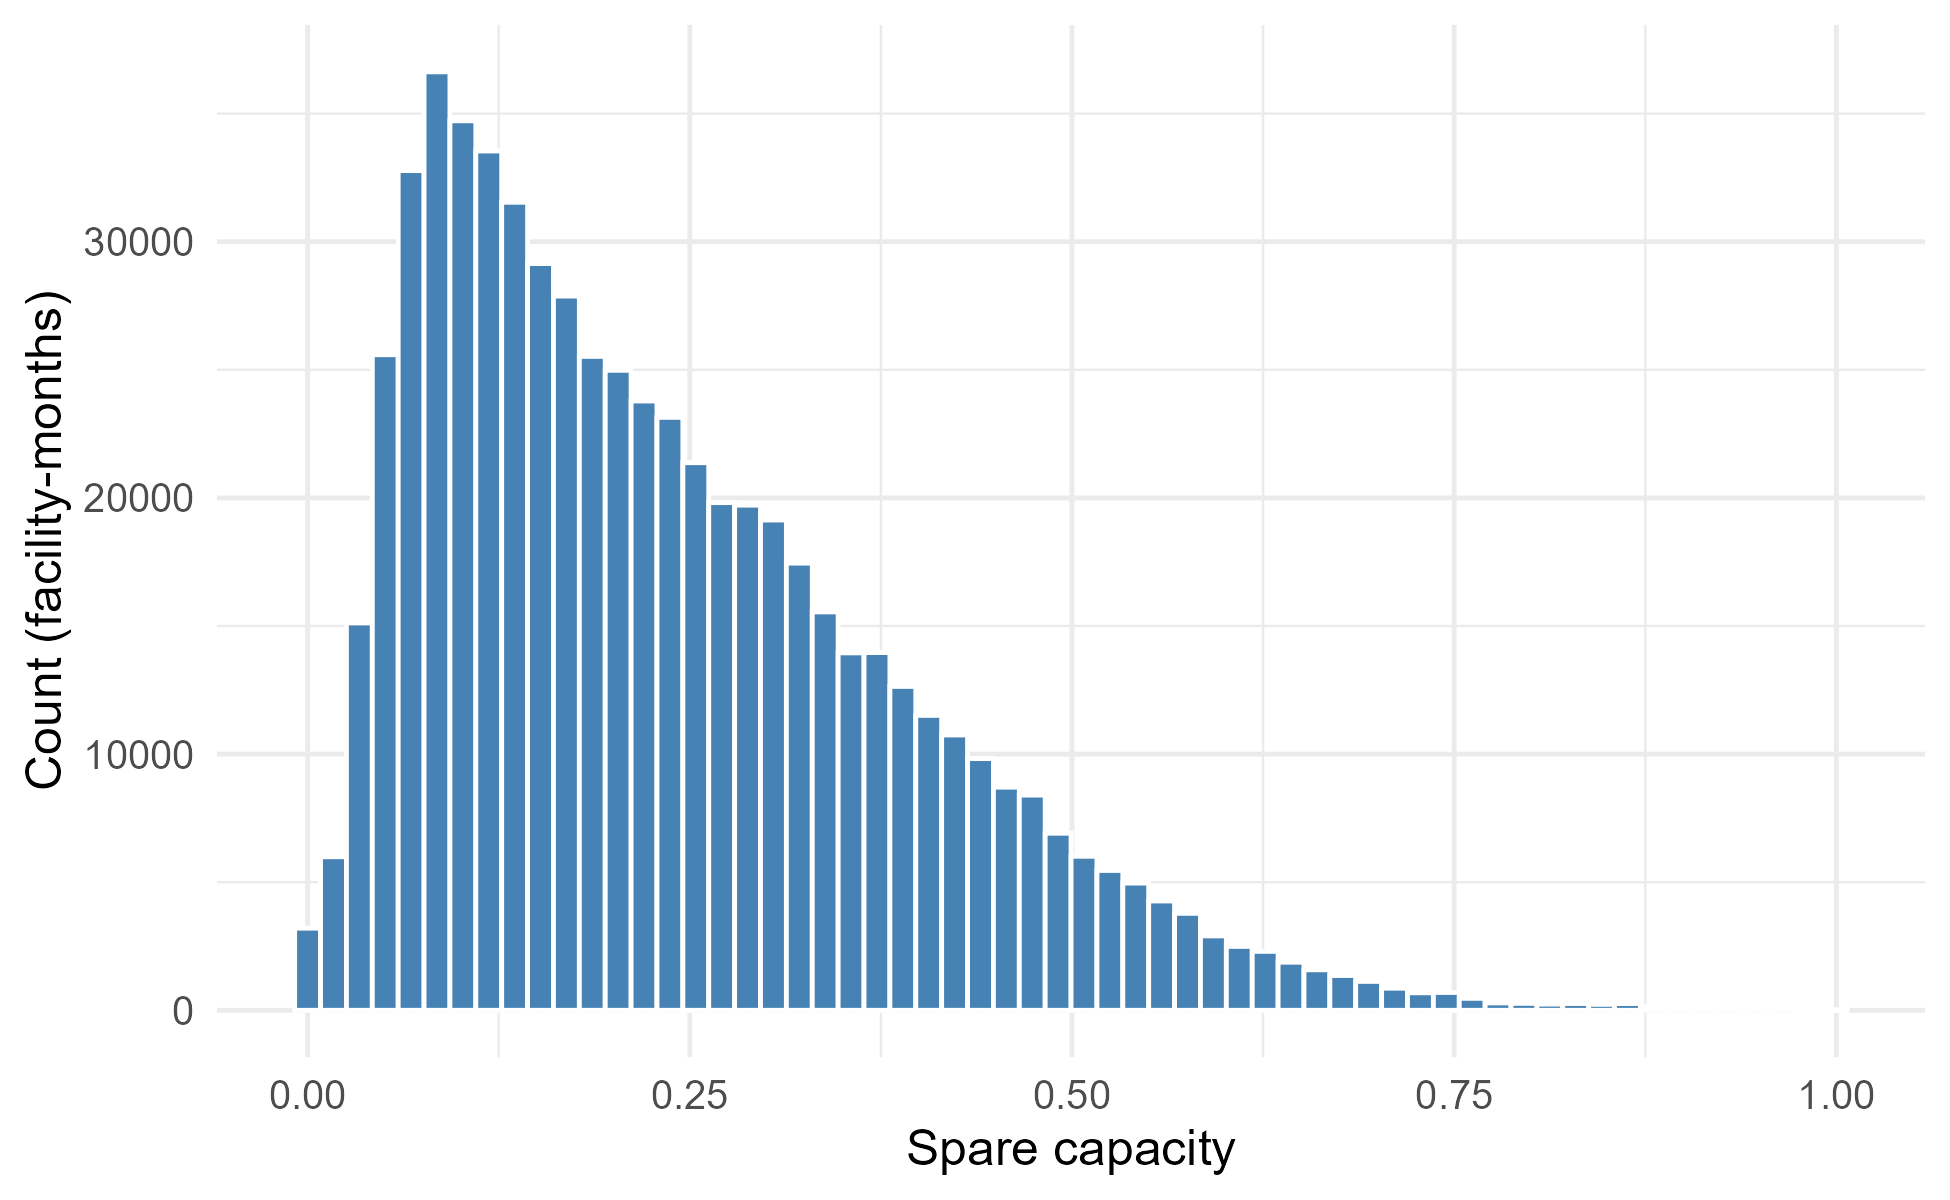
\includegraphics[width=0.8\textwidth]{spare_capacity_report_hist.png}
\caption{Distribution of Spare Capacity (Facility-Months)}
\label{fig:spare-capacity-hist}
\end{figure}

\begin{table}[H]
\centering
\begin{threeparttable}
\caption{Summary Statistics: Spare Capacity}
\label{tab:spare-capacity-summary}
\small
\setlength{\tabcolsep}{6pt}
\begin{tabular}{l r}
\toprule
\textbf{Statistic} & \textbf{Spare Capacity} \\
\midrule
N & 626,311 \\
Mean & 0.236 \\
SD & 0.155 \\
Min & 0.000 \\
P25 & 0.111 \\
Median & 0.203 \\
P75 & 0.329 \\
Max & 0.999 \\
\bottomrule
\end{tabular}
\begin{tablenotes}[flushleft]
\footnotesize
\item \textit{Notes:} Sample excludes the anticipation window.
\end{tablenotes}
\end{threeparttable}
\end{table}

\vspace{1em}

% ---------------------------------------------------------------------------
% Near-capacity vs. slack-capacity static regression (transposed)
% ---------------------------------------------------------------------------

\begin{table}[H]
\centering
\begin{threeparttable}
\caption{Spare Capacity and Occupancy Response to Ownership Change: Near-Capacity vs. Slack-Capacity Acquisitions}
\label{tab:spare-capacity-near-vs-slack-transposed}
\small
\setlength{\tabcolsep}{6pt}
\begin{tabularx}{\textwidth}{@{} l Y Y @{}}
\toprule
 & \textbf{Spare capacity} & \textbf{Occupancy rate} \\
\midrule
Slack-capacity: \textit{post} & \makecell[c]{$-0.0423^{***}$ \\ $(0.0057)$} & \makecell[c]{$\phantom{-}4.1610^{***}$ \\ $(0.5692)$} \\
Difference (Near $-$ Slack): \textit{post} $\times$ Near-capacity & \makecell[c]{$\phantom{-}0.0238^{***}$ \\ $(0.0066)$} & \makecell[c]{$-2.3312^{***}$ \\ $(0.6562)$} \\
Near-capacity effect: \textit{post} $+$ interaction & \makecell[c]{$-0.0185^{***}$ \\ $(0.0048)$} & \makecell[c]{$\phantom{-}1.8298^{***}$ \\ $(0.4793)$} \\
\midrule
Observations & 117,863 & 117,863 \\
\bottomrule
\end{tabularx}
\begin{tablenotes}[flushleft]
\footnotesize
\item \textit{Notes:} Sample restricted to ever-treated facilities, split at the median pre-acquisition spare capacity (average spare capacity over event\_time $\in [-12,-4]$, prior to the anticipation window).
\item Near-capacity $=$ baseline spare capacity $\leq$ 0.261 (median); Slack-capacity $=$ above. $N = 1443$ treated facilities with a usable baseline (722 near-capacity, 721 slack-capacity).
\item Controls exclude occupancy rate and spare capacity from each other's controls. All models include facility and calendar-month fixed effects; anticipation window excluded.
\item Standard errors are clustered two ways by facility and calendar month. Statistical significance: $^{***}p<0.01$, $^{**}p<0.05$, $^{*}p<0.10$.
\end{tablenotes}
\end{threeparttable}
\end{table}

\end{document}
